\documentclass[reqno,11pt]{amsart}
\usepackage[margin=1in]{geometry}                				% See geometry.pdf to learn the layout options. There are lots.
\geometry{letterpaper}                   						% ... or a4paper or a5paper or ... 
%\geometry{landscape}                						% Activate for for rotated page geometry
\usepackage[parfill]{parskip}    							% Activate to begin paragraphs with an empty line rather than an indent
\usepackage{subfig}
\usepackage{graphicx}
\usepackage{amssymb, amsmath}
\usepackage{epstopdf}
\usepackage[english]{babel}
\DeclareGraphicsRule{.tif}{png}{.png}{`convert #1 `dirname #1`/`basename #1 .tif`.png}
\newcommand{\tab}{\hspace*{2em}}
\begin{document}
\title{ The SIR Epidemic Model: \\
          The Deterministic and Stochastic Cases}
\author{Larry Hernandez}
\date{December 21, 2011}                                           			% Activate to display a given date or current date if no argument is provided
\maketitle
\section{Introduction}

	The spread of disease within a population depends not only upon disease-related factors such as the infectious agent, transmission modes, periods of incubation and infection, susceptibility, and resistance, but also on social, economic, demographic, geographic and other nondisease-related factors. Knowledge about a communicable disease can be gained through the study of mathematical models which incorporate these factors. Compartmental models are particularly useful for this. In these models individuals are allocated into mutually exclusive classes (compartments) based on categories of interest or epidemiological relevance and with assumptions about the nature and time rate of transfer from one compartment to another. Individuals within each compartment are considered identical in terms of their status with respect to the disease. For sufficiently large populations, differential equations can be derived to describe the time evolution of the number of individuals in each compartment. However, in the case of smaller population sizes where a system of differential equations will not feasibly describe population dynamics, a stochastic model can be formulated, analyzed, and simulated to study the time evolution of the compartments. In this paper, a well-known communicable disease model is reviewed in both its deterministic and stochastic frameworks. Modeling assumptions, terminology, notation, theorems, and numerical simulations are provided.


	The Susceptible-Infected-Removed (SIR) model is used to describe diseases such measles, chickenpox, and influenza that confer immunity against re-infection. It has been studied extensively, formulated with different assumptions, and been extended in several ways to incorporate additional compartments to analyze population dynamics for infectious human, animal, and plant diseases. For an SIR model in its most basic form, the population is characterized by three states, or compartments, which include the following:

\begin{itemize}
	\item \textit{Susceptible}: individuals who have no immunity to the infectious agent and might become infected if exposed to it.
	\item \textit{Infectious}: individuals who are currently infected and who can transmit the infection to susceptible individuals with whom they come into contact. These individuals are also labeled infectives.
	\item \textit{Removed}: individuals who are immune to infection and, therefore, do not affect the transmission dynamics whenever they come into contact with other 
		individuals. Specifically, they do not spread the disease to others. This compartment is also known as \textit{recovered} or \textit{immune} in the literature.
\end{itemize}

It is traditional to denote the number of individuals in each of the compartments by \textit{S}, \textit{I}, and \textit{R}, respectively, and common to assume that the population size,
$N$, is a constant so that for all times $N = S+I+R$. For diseases in which the average infection period is short compared to the average individual lifetime (i.e. about one week for measles), then it is safe to assume that the host population is constant in the timescale of the disease outbreak.  Another assumption that has been commonly made for the SIR model, and which we will adopt here, is that mixing between individuals is homogeneous. Of course, these assumptions can be revised to address any particular situation. The simple schematic below illustrates the SIR model just described:
\begin{equation*}
 S \rightarrow  I \rightarrow  R
\end{equation*}


	The SIR process can be modeled deterministically with differential equations and stochastically using elements from probability theory. In the stochastic case one may use a
Discrete Time Markov Chain (DTMC), a Continuous Time Markov Chain (CTMC), and/or a set of Stochastic Differential Equations (SDE). In this paper, we study the `epidemic' process, for which we mean that the number of infected cases initially increases (or even escalates) before the population becomes disease-free. We do not study the endemic case in which disease persists within a population. Our formalism includes the deterministic and stochastic CTMC settings. Study of the model through SDEs is excluded here, and the reader is referred to the literature (Allen 2008) for more information.


	We will see that the stochastic and deterministic SIR processes differ in their asymptotic dynamics. Whereas in the deterministic case the system can predictably undergo or avoid an epidemic from the start, the stochastic solution exhibits only a probability for the occurence of an epidemic. Three characteristics that are unique to the stochastic models and that will be explored are: (1) the probability of an epidemic occurring, (2) the final size distribution of an epidemic should one occur, and (3) its expected duration.
%
%
%%%%%%%%%%%%%%%%%%%%%%%%		THE DETERMINISTIC SIR MODEL		%%%%%%%%%%%%%%%%%%%%%%%%%%%
%
%
\section{The Deterministic SIR Model}

	For the deterministic version of the SIR model a set of differential equations is used to decribe how the sizes of the compartments change over time. The independent variable is
time $t$, and the dependent variables are the state variables $S(t)$, $I(t)$, and $R(t)$. Each of these variables is continuous.
%
%
%%%%%%%%%%%%%%%%%%%%%%%%		THE KERMACK-MCKENDRICK MODEL		%%%%%%%%%%%%%%%%%%%%%%%%%%%
%
%
\subsection{The (Classic) Kermack-McKendrick Model}
	The classical or ``standard" SIR epidemic model is a set of three coupled nonlinear ordinary differential equations and was first formulated by W.O. Kermack and A.G. McKendrick in 1927 to explain the rise and fall in the number of individuals infected by contagious diseases such as the plague and cholera. We assume a constant population size (i.e. no births or deaths), an instantantious incubation period of the infection, an infectious period equal to the period that an individual has the disease, and a uniformly mixing population. Based on these modeling assumptions, the system of differential equations describing the dynamics of the population are formulated as:
\begin{subequations}\label{SIR_ODEs}
\begin{align}
\frac{dS}{dt} &= -\frac{\beta}{N} S I \label{SIR_dSdt} \\
\frac{dI}{dt} &= \frac{\beta}{N} SI - \gamma I \label{SIR_dIdt} \\
\frac{dR}{dt} &= \gamma I \label{SIR_dRdt}
\end{align}
\end{subequations}

where $\beta > 0 $ is the \textit{contact rate} or \textit{transmission rate} and $\gamma > 0$ is the \textit{recovery rate} or \textit{removal rate} of the infectives. The value $1/ \gamma $ is the average period of infection. The parameter $\beta$ represents the number of contacts that result in an infection of a susceptible individual by one infective. The contact rate may be a function of population size N (i.e. $\beta = cN$ for some constant c), a constant, or take on some other form. If the population size is not constant, then the form of $\beta$ can have a significant impact on the population dynamics (Allen 2003). In this paper, however, we consider only the case of constant $ \beta $. Although this model is very simple, it is useful in making relevant general comments about epidemics and can be used to adequately describe some specific epidemics. 


The formulation of the deterministic model is complete when given initial conditions, such as $S(0)$, $I(0)$, $R(0) \ge 0$, and $S(0) + I(0) + R(0) = N$. In the examples, we mainly consider the case when $R(0) = 0$ and $I(0) = 1$.


Natural questions to pose for any epidemic are: Given the parameters $\beta$, $\gamma $ and initial conditions $S(0) = S_0$, $I(0) = I_0$, and $R(0)=R_0$, will the infection spread or will it die out? Also, if it does spread, how many individuals will be affected? With some mathematical analysis, which comes from Murray, we can determine answers to these questions.


\subsection{Threshold for Epidemic}
	We are only interested in nonnegative solutions for $S(t)$, $I(t)$, and $R(t)$; otherwise, they would not be epidemiologically meaningful since these variables represent numbers of people within categories. 


	First, it can be seen from equation \eqref{SIR_dIdt} that:

\begin{equation*}
\left [ \frac{dI}{dt} \right ] \bigg| _{t = 0}= I_0 \left( \frac{\beta}{N} S_0 - \gamma \right ) \begin{cases}
> 0 & 	\text{ if $ S_0 > \rho $}, \\
< 0 & 	\text{ if $ S_0 < \rho $} \\
\end{cases}
\end{equation*}

where $\rho = \frac{\gamma N}{\beta}$ is termed the \textit{relative removal rate}. From equation \eqref{SIR_dSdt} we see that $\frac{dS}{dt} \le 0$, implying that $S \le S_0$, so that if 
$S_0 < \rho $, then:

\begin{equation*}
\left [ \frac{dI}{dt} \right ] = I \left ( \frac{\beta}{N} S - \gamma \right ) \le 0 \text{\tab \tab for all $t \ge 0$} 
\end{equation*}


which means that $I_0 > I(t) \rightarrow 0$ as $t \rightarrow \infty$. In this case, the infection dies out and there is no epidemic! In the case that $S_0 > \rho $, then $I(t)$ initially increases and there is an epidemic. Recall that by 'epidemic' we mean $I(t) > I_0$ for some $t > 0$. Thus, there is a threshold phenomenon that exists for the SIR model. When $S_0 > \rho $ there is an epidemic; whereas, if $S_0 < \rho $ there is no epidemic.
%
%
%%%%%%%%%%%%%%%%%%%%%%%%		THE REPLACEMENT NUMBER				%%%%%%%%%%%%%%%%%%%%%%%%%%%%
%
%
\subsection{The Replacement Number, \textit{R}} An important parameter to the SIR model is the \textit{effective reproduction number} or \textit{replacement number} and is defined by Allen (2003) as

\begin{equation}
\begin{split}
    R& = \frac{S_0}{N}\frac{\beta}{\gamma} \\
      & = \frac{S_0}{N} R_0
\end{split}
\end{equation}

	The replacement number, \textit{R}, gives the average number of secondary infections that a typical infective produces during the entire period of infectiousness. The parameter $R_0  = \frac{\beta}{\gamma} $ is termed the \textit{basic replacement number} (Hethcote 2000) and represents the average number of secondary infections that occur when one infective is introduced to a completely susceptible population. As seen above, the threshold for an epidemic is related to the relative removal rate $\rho$. If $S_0 > \rho$ then an epidemic occurs, but if $S_0 < \rho$ then there is no epidemic. It is common to state this threshold in terms of the effective replacement number $R = \frac{S_0 \beta}{N \gamma} $. If $R \le 1$ then there is no epidemic. However, if $R > 1 $  then an epidemic occurs.
%
%
%%%%%%%%%%%%%%%%%%%%%%%%		EXAMPLE 1: EPIDEMIC AND NO EPIDEMIC 		%%%%%%%%%%%%%%%%%%%%%%%%%%%
%
%
\subsection{Example} A numerical simulation is performed to solve equations \eqref{SIR_ODEs} describing the SIR model for the case when $\beta = 2$, $ \gamma = 1$, $I(0) = 1$, $N=100$ so that $R = 1.98$ and hence an epidemic occurs. A plot of the time rate of change of the susceptible and infected compartments is included in figure~\ref{fig:Epidemic}. Since $R>1$ the number of infectives initially increases before reaching a maximum, after which it decreases to zero.

For completeness, an instance in which no epidemic occurs is illustrated in figure~\ref{fig:NoEpidemic}. One sees that the number of infectives immediately decreases to zero as expected.

\begin{figure}[ht]
\begin{center}
\subfloat[Epidemic]{\label{fig:Epidemic}
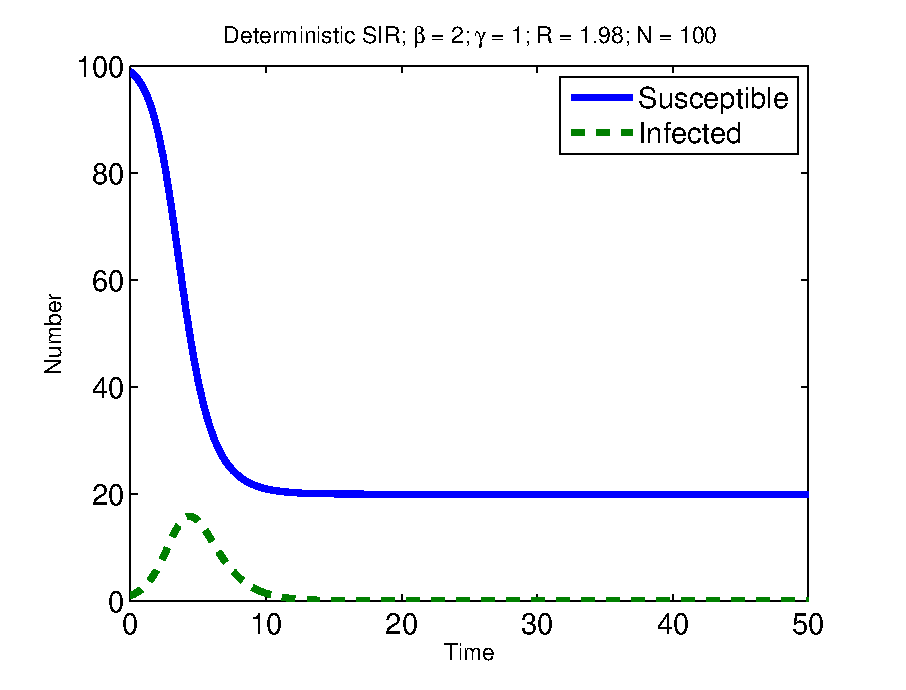
\includegraphics[height=3in,width=3.5in]{Determ_Epidemic.eps}
}
\subfloat[No epidemic]{\label{fig:NoEpidemic}
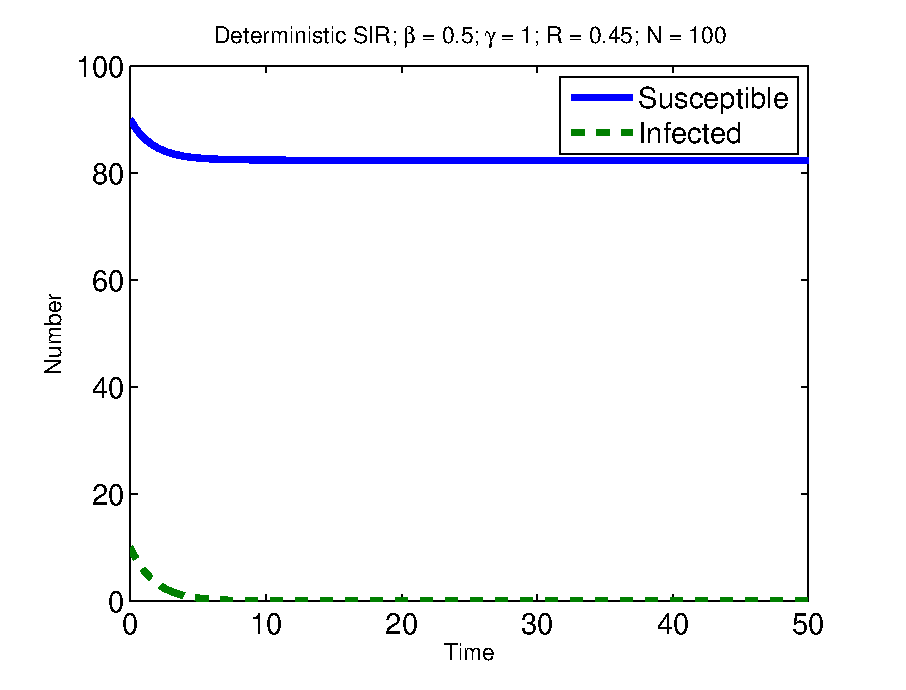
\includegraphics[height=3in,width=3.5in,angle=0]{Det_NoEpi_I010.eps}
}
\caption{Deterministic SIR Model}
\end{center}
\end{figure}



%\begin{figure} 
%\begin{center} 
%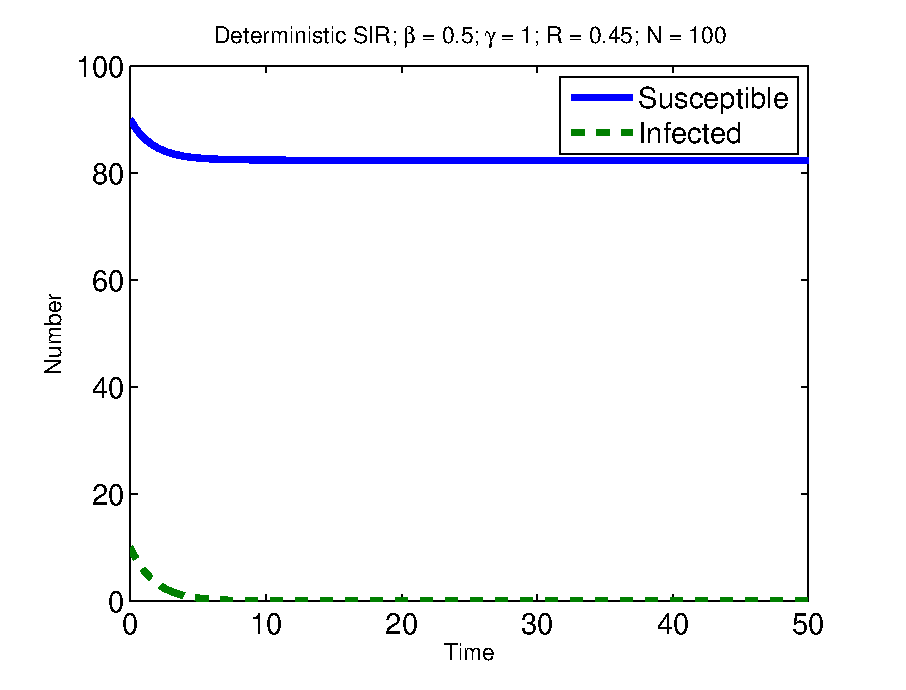
\includegraphics[height=3in,width=3in,angle=0]{Det_NoEpi_I010.eps} 
%\caption{\small \sl No epidemic for deterministic SIR with  .\label{fig:Det_NoEpi}} 
%\end{center} 
%\end{figure}  
%
%
%%%%%%%%%%%%%%%%%%%%%%%%			SEVERITY OF THE EPIDEMIC			%%%%%%%%%%%%%%%%%%%%%%%%%%%
%
%
\subsection{Severity of the Epidemic}
If an epidemic occurs then we would like to know how severe it will be. That is, how many people will the disease affect? To begin the calculation, we divide equation \eqref{SIR_dIdt} by equation \eqref{SIR_dSdt}, obtaining the following differential equation for \textit{I} in terms of \textit{S}:
\begin{equation}\label{PhaseSpaceODE}
      \frac{dI}{dS}  =  \frac{\frac{\beta}{N} S I - \gamma I}{- \frac{\beta}{N}SI} = -1 + \frac{N \gamma}{\beta S},  \text{\tab \tab $S > 0$}
\end{equation}

for which we see that the line $I = 0$ contains all singularities. 

Separating variables, integrating, and applying the initial conditions yields the following $(I,S)$ phase plane trajectories:
\begin{equation}\label{PhaseSpaceTrajectories}
I(t) + S(t) - \rho \text{ } ln\left ( S(t) \right ) = I(0) + S(0) + \rho \text{ } ln \left( S(0) \right) = \text{a constant}
\end{equation}

where we have used the initial condition $I(0) + S(0) = N$.

Next, we notice that when an epidemic occurs, then equation \eqref{PhaseSpaceODE} tell us that $I_{max}$, the maximum value of $I$, occurs when $\frac{dI}{dt} = 0 $, which corresponds to $S = \rho $. Inserting this value of $S$ into equation \eqref{PhaseSpaceTrajectories} yields:
\begin{equation}\label{Eq_Imax}
\begin{split} 
I_{max} & = \rho \text{ } ln ( \rho ) - \rho + I_0 + S_0 - \rho \text{ } ln ( S_0 ) \\
      & = I_0 + ( S_0 - \rho ) + \rho \text{ } ln \left ( \frac{ \rho }{ S_0 } \right ) \\	
      & = N - \rho + \rho \text{ } ln \left ( \frac{\rho}{S_0} \right )
\end{split}
\end{equation}

For any set of initial values $I_0 > 0$ and $S_0 > \rho$, the value $I$ increases from $I_0$ and hence we have an epidemic on our hands. The severity of the epidemic will depend on how close $I_0$ is to $I_{max}$. Additionally, we see that if $S_0 < \rho$ then $I$ decreases from $I_0$ and there is no epidemic. We restate this result in terms of the replacement number $ R$: 

\textit{For the deterministic Kermack-McKendrick SIR model described by equations \eqref{SIR_ODEs}, if $R \le 1$ then solutions $I(t)$ decrease monotonically to zero and there is no epidemic. However, if $R > 1 $  then $I(t)$ increases before it decreases to zero and an epidemic occurs}.

We continue to use the $(I,S)$ phase plane and equations \eqref{SIR_ODEs} to analyze the long-term behavior of $I(t)$ and $S(t)$. Because $I = 0 $ is a line of singularities, then for all trajectories in the $(I,S)$ phase plane we have that $I(t) \rightarrow 0$ as $t \rightarrow \infty$. Also, since $\frac{dS}{dt} < 0$ for $S \ne 0, I \ne 0$, then S(t) is a decreasing function. We get from equations \eqref{SIR_dSdt} and \eqref{SIR_dRdt} that:

\begin{equation}
\begin{split}
& \frac{dS}{dR} = - \frac{S}{\rho} \\
& \Rightarrow 	S(t) = S_0 \text{ } exp \left [- \frac{R(t)}{\rho} \right ] \ge S_0 \text{ } exp \left [- \frac{N}{\rho} \right ] > 0 \\
\label{Bound_S}
& \Rightarrow	0 < S(\infty) \le N
\end{split}
\end{equation}


Combining the fact that $I(\infty) = 0$ and $S(t) + I(t) + R(t) = N$ for all times, we obtain $R(\infty) = N - S(\infty)$. We then substitute this result into \eqref{Bound_S} to gain an expression for $S(\infty)$:
\begin{equation}\label{S_trans}
S(\infty) = S_0 \text{ } exp \left [ - \frac{N - S(\infty)}{\rho} \right ]
\end{equation}

We now have that $S(\infty)$ is the positive root of transcendental equation \eqref{S_trans}, which is the total number of susceptibles who did not catch the disease during the epidemic. We can now easily calculate the total number of susceptibles who catch the disease during the entire course of the epidemic:
\begin{equation*}
I_{total} = I_0 + S_0 - S(\infty)
\end{equation*}

As a note, the total number of susceptibles who have caught the disease, $I_{total}$, are also denoted by $R(\infty)$. This analysis has shown that as $t \rightarrow \infty$, $I(t) \rightarrow  0$ and $S(t) \rightarrow S(\infty) > 0$. The disease will die out due to a lack of infectives rather than due to a shortage of susceptible individuals!
%
%
%%%%%%%%%%%%%%%%%%%%%%%%                   EXAMPLE DETERMINISTIC CASE: FINAL SIZE                          %%%%%%%%%%%%%%%%%%%%
%
%
\subsection{Example} We calculate the final size, $R(\infty)$, of an SIR epidemic when $ \gamma =1$, $S(0) = N - 1 $, and $I(0)=1$. The results are included in table~\ref{Table_DetFinalSize}. It can be seen that when $R \le 1$, or equivalently when $\beta \le 1$, there is no epidemic. The final size of the epidemic is quite small; however, as $\beta$ increases and exceeds unity, then an epidemic ensues. The final size of the epidemic increases as $\beta$ (i.e. $R$) increases. For $\beta = 10$, a total outbreak has occurred and everybody in the population contracts the disease.
\begin{table}[ht]
	\begin{tabular}{|c||ccc|}
		\hline
	 	   &           &    N       &			\\ \cline{2-4}
	$\beta$ &  $20$ & $100$  	& $1000$   		\\
	\hline
	0.5 & 1.87	& 1.97 		& 2.00   	\\
	1   & 5.74 	& 13.52 	& 44.07  		\\
	2   & 16.26 	& 80.02 	& 797.15 		\\
	5   & 19.87 	& 99.31 	& 993.03  		\\
	10  & 20 	& 100 		& 999.95  		\\
	\hline
	\end{tabular}
	\caption{Deterministic SIR: Final Size of Epidemic}
	\label{Table_DetFinalSize}
\end{table}
%\begin{figure} 
%\begin{center} 
%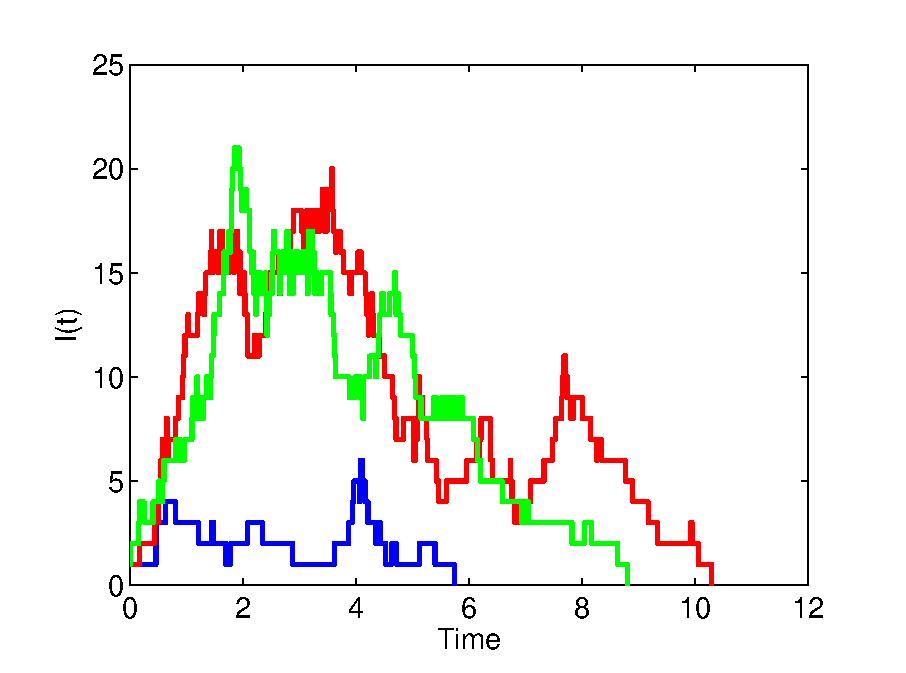
\includegraphics[height=3in,width=3in,angle=0]{Fig_SIR_Gillespie.eps} 
%\caption{\small \sl Three realizations of the stochastic SIR model .\label{fig:SochasticSIR}} 
%\end{center} 
%\end{figure}
%
%
%%%%%%%%%%%%%%%%%%%%%%%%		LIMITATIONS OF THE DETERMINISTIC MODEL	%%%%%%%%%%%%%%%%%%%%%%%%%%%
%
%
\subsection{Limitations of the Deterministic Model}
We have shown that in the deterministic SIR setting, the value of $\mathcal R$ (equivalently, $ \rho$) determines the occurrence of an epidemic. The results rely on the assumption that the population is homogeneous and that mixing of individuals occurs uniformly. This of course is not realistic, as we know that mixing depends on several factors, such as age---for example, children typically engage in a higher rate of mixing per day than adults. Additionally, different geographic, cultural, and socio-economic groups will exhibit different rates of contact. 

For cases in which homogeneous mixing can be assumed accurate, it is still reasonable to assume that the classic SIR model is not entirely suitable. For a small population, such as a school or local community center, it is reasonable to suppose uncertainty in the final number of individuals infected by the disease. Better yet, one may consider the idea that for $R_0 > 1$---the condition guaranteeing the occurrence of an epidemic---and a large population that if only a few individuals or even just one individual is infected at the onset, it may be possible for an epidemic to not ever escalate! This is a realistic situation which motivates the formulation of a stochastic version of the SIR model.

As a last note, the deterministic model, which considers the state variables $S$, $I$, and $R$ to be continuous, is suitable in the regime of large population sizes. This is unrealistic for small populations.
%
%
%
%%%%%%%%%%%%%%%%%%%%%%			THE STOCHASTIC SIR MODEL			%%%%%%%%%%%%%%%%%%%%%%%%%%
%
%
%
\section{Stochastic SIR Model}
The stochastic epidemic process can be defined with the use of a Continuous Time Markov Chain. In this setting, time is a continuous variable with time scale, $t \in [0, \infty]$, and the states $\mathcal S(t), \mathcal I(t),$ and $\mathcal R(t)$ are discrete random variables for the number of susceptible, infected, and immune individuals, respectively:
\begin{equation*}
\mathcal S(t), \mathcal I(t), \mathcal R(t) \in \lbrace 0, 1, 2, ...,N \rbrace
\end{equation*}
where $\mathcal S(t) + \mathcal I(t) + \mathcal R(t) = N$. The population is assumed to mix homogeneously. There is no latent period so that infectives are immediately infectious to others. Similar to the deterministic case considered above, we assume that infecteds recover from the disease and develop permanent immunity. Vital dynamics are not considered in this formulation, so that there are no births or deaths during the process, and the population size, $N$, is constant. Consequently, there are only two independent variables $\mathcal S(t)$ and $\mathcal I(t)$, since $\mathcal R(t) = N - \mathcal S(t) - \mathcal I(t)$. The stochastic SIR model is a bivariate process $\lbrace (\mathcal S(t), \mathcal I(t)) \rbrace _{t=0}^\infty$ with a joint probability function given by
\begin {equation}\label{SIR_JointPDF}
p_{(s,i)}(t) = Pr \lbrace \mathcal S(t) = s, \mathcal I(t) = i \rbrace
\end {equation}


% In the DTMC epidemic model, $t \in \lbrace 0, h, 2h,...\rbrace$ for some (small) time step $h$, and the discrete random variables for the states satisfy
%\begin{equation*}
%\mathcal S(t), \mathcal I(t), \mathcal R(t) \in \lbrace 0, 1, 2, ...,N \rbrace
%\end{equation*}

%The transition probabilities can be defined based on the assumptions of the SIR model. First we assume that $h$ can be chosen sufficiently small so that at most one change in state occurs during the time interval $h$. That is, there can be either a new infection, a birth, a death, or a recovery in time increment $h$. The transition probabilities from the state $(\mathcal S(t), \mathcal I(t)) = (s,i)$ to state $(\mathcal S(t+h), \mathcal I(t+h)) = (u,v)$, $(s,i) \rightarrow (u,v)$ are denoted by the following notation:
%\begin{equation*}
%p_{( u,v ),(s,i)} (h) = Pr \lbrace ( \mathcal S(t+h) = u , \mathcal I(t+h) = v ) | (\mathcal S(t), \mathcal I(t)) = (s,i) \rbrace
%\end{equation*}
%
%with the transition probabilities given by:
%\begin{equation*}
%p_{( u,v ),(s,i)} (h) = \begin{cases} 
%(\beta is/N)h&	\text{if $(u,v)=(s-1,i+1)$}, \\  				% new infection
%\gamma ih&	\text{if $(u,v)=(s,i-1)$}, \\					% death or recovery		
%bih&		\text{if $(u,v)=(s+1,i-1)$}, \\				% ?
%b(N-s-i)h&	\text{if $(u,v)=(s+1,i)$}, \\					% birth
%1-\beta is/Nh - [\gamma i + b(N-s)]h& \text{if $(u,v)=(s,i)$}, \\		% no change
%0&		\text{otherwise}
%\end{cases}
%\end{equation*}
%
%The probability of a new infection, $(s,i)\rightarrow(s-1,i+1)$, is.... The probability of a death or recovery, INSERT TRANSITION NOTATION, is 
%
%
%The time step $h$ must be sufficiently small that each of the transition probabilities lies in the inteval [0,1]. Now, the states of the system are ordered pairs $(s,i)$, so that the form of the transition matrix Q depends on how the states are ordered. Luckily, we can use the Markov property and write the difference equation for the probability $p_{(s,i)} (t+h)$ in terms of the transition probabilities:
%\begin{equation*}
%\begin{split}
%p_{(s,i)} (t+h) &= p_{(s+1,i-1)} (t) \frac{\beta}{N} (i-1)(s+1)h + p_{(s,i+1)} (t) \gamma (i+1)h \\ 
%                        & + p_{(s-1,i+1)} (t) b (i+1)h+ p_{(s-1,i)} (t) b (N-s+1-i)h \\
%		& + p_{(s,i)} (t) \left( 1- \left [ \frac{\beta i s }{N} + \gamma i + b (N-s) \right ] h \right ).  
%\end{split}
%\end{equation*}
%It is fairly intuitive to see that the state $(\mathcal S(t), \mathcal I(t)) = (N,0)$ is absorbing and that all other states are transient. That is, all sample paths are eventually absorbed into the disease-free state $(N,0)$ regardless of the magnitude of the basic reproduction number $R_0$. This is a major difference from the deterministic setting in which a disease-free equilibrium is achieved only when $R_0 \le 1$.
%
%
%%%%%%%%%%%%%%%%%%%%%%%%%%%	TRANSITION PROBABILITIES & FORWARD EQUATIONS      %%%%%%%%%%%%%%%%%%%%%%
%
%
\subsection{Transition Probabilities and Forward Equations}
In studying this stochastic process, we use $h$ to denote small time increments and define $\Delta \mathcal S(t) = \mathcal S(t+h) - S(t)$ to denote the change in the state variable $\mathcal S$ from time $t$ to time $t+h$. Analogous definitions are made for $\Delta \mathcal I(t)$ and $\Delta \mathcal R(t)$. We assume that $h$ is sufficiently small so that at most one change in the state occurs during the time interval. For this version of the model, this means that there can be at most one recovery or one new infection in the time interval $h$.

Using the assumptions for the stochastic SIR model, the infinitesimal transition probabilities satisfy:
\begin{equation*}
Pr \lbrace \Delta \mathcal S(t) = s, \Delta \mathcal I(t) = i | \mathcal S(t), \mathcal I(t)  \rbrace = 
\begin{cases}
	\frac{\beta}{N} \mathcal S(t) \mathcal I(t) h + o(h),  							&  \text{if $(s,i) = (-1,1)$ } 	\\
	\gamma \mathcal I(t) h+o(h),											&  \text{if $(s,i) = (0,-1)$ } 	\\
	1 - \left[ \frac{\beta}{N} \mathcal S(t)  \mathcal I(t) + \gamma \mathcal I(t) \right ] h + o(h), 		&  \text{if $(s,i) = (0,0)$ } 	\\
	o(h),														&  \text{otherwise.}
\end{cases}
\end{equation*} 

%\begin{equation*}
%\mathcal S(t), \mathcal I(t), \mathcal R(t) \in \lbrace 0, 1, 2, ...,N \rbrace
%\end{equation*}

%$$
%Pr \lbrace \Delta \mathcal S(t) = i, \Delta \mathcal I(t+h) - I(t) = j | \Delta S(t), \Delta I(t)  \rbrace =
%$$
%$$
%\begin{cases}
%	\frac{\beta}{N} S(t)I(t)h + o(h)  						&  \text{if (s,i) =(-1,1);} 	\\
%            \frac{\beta}{N} S(t)I(t)h + o(h) 						&  \text{if (s,i) =(1,0);} 	\\
%	\gamma I(t)h+o(h)								&  \text{if (s,i) =(0,-1);}	\\
%	1 - \left[ \frac{\beta}{N} S(t) I(t) + \gamma I(t) \right ] h + o(h) 		&  \text{if (s,i) =(0, 0);} 	\\
%	o(h)										&  \text{otherwise.}
%\end{cases}
%$$

where, for example, when $ \Delta \mathcal I(t) = -1 $, then $ \Delta \mathcal R(t) = 1 $. The transitions $(s,i) = (-1,1)$ represent a susceptible that has become infected, and the transitions $(s,i) = (0, -1)$ represent recovery of an infected individual. No other transitions are allowed.

We assume an initial distribution $(\mathcal S(0), \mathcal I(0)) = (s_o,i_o)$, where $s_o \ge 0$, $i_o > 0$, and $s_o+i_o=N$. We will, again, make $i_0=1$ for some examples. Using the infinitesimal transition probabilities and the joint probability distribution we can write a relationship for the time changing state probabilities:
\begin{equation*}
p_{ (s,i) } (t+h) = \frac{ \beta }{N} (s+1) (i-1) p_{ (s+1,i-1) } (t) h+ \gamma (s+1) p_{ (s,i+1) } (t) h + \left ( 1 - \left [ \frac{ \beta }{N} s i + \gamma i \right ] \right ) p_{ (s,i) } (t)  h + o(h)
\end{equation*}

Subtracting $p_{(s,i)} (t)$ from both sides and dividing by $h$ yields:
\begin{equation*}
\begin{split}
\frac{p_{(s,i)} (t+h) - p_{(s,i)} (t) }{h} &= \frac{\beta}{N} (s+1) (i-1) p_{ (s+1,i-1) } (t) + \gamma (s+1) p_{ (s,i+1) } (t) ... \\ & - \left [ \frac{ \beta }{N} s i + \gamma i \right ] p_{ (s,i) } (t)  + o(h)
\end{split}
\end{equation*}

Taking the limit $h \rightarrow 0$, we obtain the \textit{forward Kolmogorov equations} describing the state probabilities:
\begin{equation}\label{Eq_Kolmogorov}
\frac{dp_{(s,i)} (t)}{dt} = \frac{\beta}{N} (s+1)(i-1) p_{(s+1,i-1)} (t) + \gamma (s+1) p_{(s,i+1)} (t) - \left[ \frac{\beta}{N}s i  + \gamma s \right] p_{(s,i)} (t)
\end{equation}

where $ s = 0, 1, 2 ,...N$, $ i = 0, 1, 2,...,N-s $, and $ 0 \le s+i \le N$. The probabilities are assumed to be zero when $(s,i)$ do not lie within this range, as they would not be epidemiologically meaningful. Additionally, when $ i=0$ and $ s = 0,1,2,...,N-1$ we have that

\begin{equation*}
\frac{dp_{(s,0)}}{dt} = \gamma p_{(s,1)}      \text{\tab and \tab} 	\frac{dp_{(N,0)} } {dt} = 0
\end{equation*}

The N+1 ordered pairs $(s,0)$ with $ s = 0, 1,2,...N $ form a closed set of states; there are no transitions out of them to any other states. This makes sense intuitively; if there are no infectives remaining in the population, then there is no way for the disease to spread to others and the process is over. In fact, for a constant population size $N$, the stochastic process will always end up in one of the disease-free $N+1$ absorbing states! Three sample paths of the stochastic SIR model are generated and plotted in figure~\ref{fig:SIRGillespie}, demonstrating that the stochastic SIR process always ends in the absorbed state.

\begin{figure} 
\begin{center} 
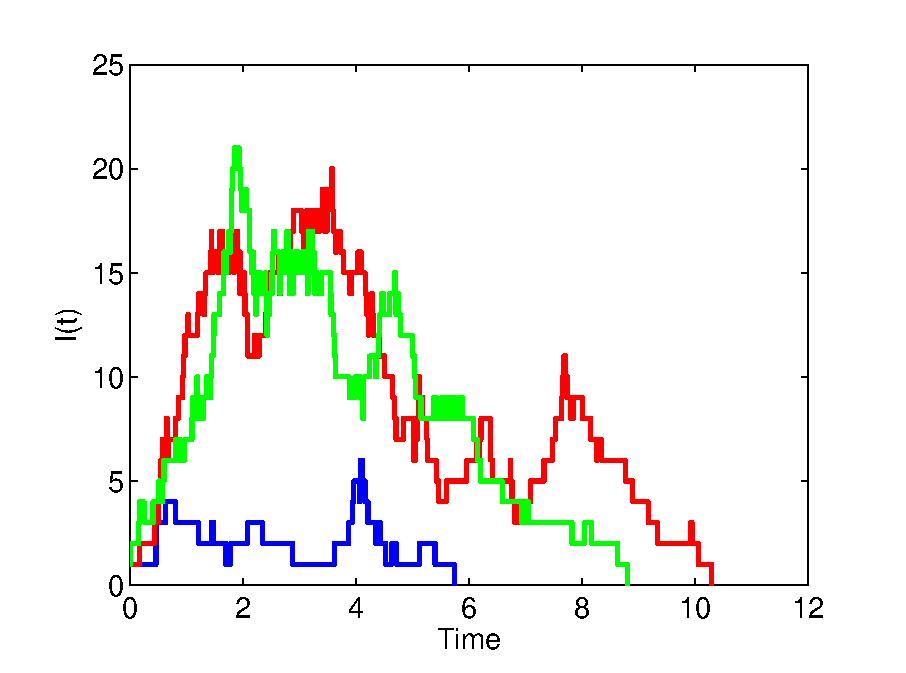
\includegraphics[height=3in,width=3in,angle=0]{Fig_SIR_Gillespie.eps} 
\caption{\small \sl Three realizations of stochastic SIR with $N=100, \beta = 2, \gamma = 1, S(0)=99$, and $I(0)=1; \mathcal R_0 = 2$\label{fig:SIRGillespie}}
\end{center} 
\end{figure}  
%
%
%%%%%%%%%%%%%%%%%%%%				STOCHASTIC SIR: Generator Matrix				%%%%%%%%%%%%%%%%%%%%%%%%
%
%
\subsection{Generator Matrix}
Although the stochastic SIR process is bivariate, we can obtain the generator matrix $A$ and transition matrix Q that correspond to the embedded Markov chain. There are $\frac{(N+1)(N+2)}{2}$ ordered pairs of states in the stochastic SIR epidemic process, and the form of matrices A and P depends on the particular ordering of these states. A useful ordering is the following:
\begin{equation}\label{StochSIR_order}
(N,0), (N-1,0),...,(0,0),(N-1,1),(N-2,1),...(0,1), (N-2,2),(N-3,2),...(0,2),...(0,N).
\end{equation}

Using this ordering, we can define:
\begin{equation*}
p(t) = (p_{(N,0)}(t),p_{(N-1,0)}(t),...,p_{(0,N)}(t) )^T
\end{equation*}
and thus are able to rewrite the forward Kolmogorov equations \eqref{Eq_Kolmogorov} as $\frac{dp}{dt}=Ap$. The generator matrix A will depend on this particular ordering of states and will have dimensions $\frac{(N+1)(N+2)}{2} \times \frac{(N+1)(N+2)}{2}$. The first $ N+1 $ columns will be all zeroes as these correspond to the $N+1$ absorbing states $(s,0)$, with $s = 0, 1, 2, ...N$, characterized by zero infectives. Again, there are no transitions away from these states.
%
%
%%%%%%%%%%%%%%%%%%				STOCHASTIC SIR: PROBABILITY OF AN EPIDEMIC			%%%%%%%%%%%%%%%
%
%	
\subsection{Probability of an Epidemic}
In the deterministic setting we know that an epidemic occurs if the replacement number $\mathcal R > 1$. In the stochastic setting, however, an epidemic can occur with a probability that is a function of the basic replacement number $\mathcal R_0$. We estimate this probability for the case when $s_0 \approx N$ and $i_0 = j$ is small. 

%When these conditions hold true, then 

We can then relate the SIR epidemic model to a simple birth and death process, where "death" corresponds to recovery in the SIR model and "birth" corresponds to  new infection. For a linear birth and death process, the probability of absorption into the 0 state depends on the parameters $\lambda , \mu$, and $x_0$, the initial state of the system, in the following way:
\begin{equation}\label{BirthDeath}
\lim _{t\rightarrow \infty} \text{Prob}{X(t) = 0}  = \begin{cases}
1, \text{ \tab \tab \tab $\lambda \le \mu $ },\\
\left ( \frac{\mu}{\lambda} \right ) ^{x_0} \text{\tab \tab   $\lambda > \mu $}
\end{cases}
\end{equation}


At the beginning of the epidemic, when $\mathcal I(0) = j$ is small, $\mathcal S(0) = N - j \approx N$, so that $\mathcal R \approx \mathcal R_0$. Substituting $\gamma$ for $\mu$ and $\beta$ for $\lambda$ in \eqref{BirthDeath}, the probability that an epidemic either ends quickly or simply does not occur can then be approximated using:
\begin{equation}
\text{Probability of no epidemic} = \begin{cases}
1, \text{ \tab \tab \tab $\mathcal R_0 \le 1$ },\\
\left ( \frac{1}{\mathcal R_0} \right ) ^j \text{\tab \tab $\mathcal R_0 > 1$}
\end{cases}
\end{equation}

These results can be reformulated as probabilities that an epidemic does occur:

\begin{equation}
\text{Probability of an epidemic} = \begin{cases}
0, \text{\tab \tab \tab $\mathcal R_0 \le 1$} \\
1- \left ( \frac{1}{\mathcal R_0} \right ) ^j , \text{ \tab $\mathcal R_0 > 1$}
\end{cases}
\end{equation}

The approximation improves as N increases and for smaller initial number of infectives $i_0$. Since we know that in the stochastic setting the system eventually ends up in the absorbed state characterized by disease-free equilibrium, these estimated probabilities apply only for a range of times $t \in \lbrace T_1, T_2 \rbrace$, which can be long when $N$ is large and $I_0$ is small.
%
%
%%%%%%%%%%%%%%%%%%%%				STOCHASTIC SIR: Transition Matrix				%%%%%%%%%%%%%%%%%%%%%%%%
%
%
\subsection{Transition Matrix}
Recalling that we have chosen to order the states of the embedded Markov chain according to \eqref{StochSIR_order}, we group the states into $N+1$ sets as follows:

\tab \tab \tab $1: (N,0), (N-1,0), (N-2,0), (N-3,0),(N-4,0), ...(1,0), (0,0)	$ %		\\

\tab \tab \tab \tab $ 2: (N-1,1), (N-2,1), (N-3,1)...,(2,1), (1,1), (0,1)	$ %		\\

\tab \tab \tab \tab \tab $ 3: (N-2,2), (N-2,2),...(2,2), (1,2), (0,2)		$	%	\\

\tab \tab \tab \tab \tab \tab . 	    	 					%	\\

\tab \tab \tab \tab \tab \tab  \tab   . 	     						%	\\

\tab \tab \tab \tab \tab \tab  \tab \tab $ N: (1,N-1), (0,N-1)$					%\\

\tab \tab \tab \tab \tab \tab  \tab \tab \tab $ N+1: (0,N) $						% \\

The transition matrix Q of the embedded Markov chain then has the follwing block form:
\begin{equation}
Q = 
\begin{bmatrix}
I&    	A_1&     	0&     		0&     		0&... 		\\
0&    	0&        	A_2& 		0& 		0&... 		\\
0& 	B_1& 		0& 		A_3&  		0&... 		\\
0& 	0& 		B_2& 		0&  		A_4&... 	\\
0& 	0& 		0& 		B_3&  		0&... 		\\
0&	0&		0&		0&		B_4&... 	\\
.&	.& 		.&		.&		.&...		\\
.&	.&		.&		.&		.&...		\\
\end{bmatrix}
\end{equation}
and corresponds to the collection of the states into $N+1$ groups. Each of the block matrices $A_j$ and $B_j$ have different dimensions and represent different transitions between the sets. The upper left corner is an $N+1 \times N+1$ identity matrix, corresponding to the first N+1 states $(s,0)$ for $s = 0, 1, 2,...,N $ which are absorbing. The $A_j$ represent recovery, transitions from $ j $ infected individuals to $ j-1 $ for $ j = 1, 2, 3,...N $, and the $B_j$ represent infection, transitions from j infected individuals to $ j +1 $  infected individuals. 

To calculate the transition matrix elements for the $A_j$ and $B_j$, we recall transitions to $(s,i-1)$ represent recovery of an infected, transitions from state $(s,i)$ to $(s-1, i+1)$ represent a susceptible that becomes infected, and that there are no other transitions. In the first type of transition, the probability of recovery is:
\begin{equation}\label{probrecovery}
p_s = \frac{ \gamma i}{ \gamma i + \left (\beta /N \right ) i s} = \frac{ \gamma }{ \gamma + \left ( \beta / N \right ) s}, \text{\tab $s = 0,1,2,...N-1$}
\end{equation}

For the second type of transition, a susceptible individual becomes infected with a probability
\begin{equation}\label{probinfection}
1-p_s = \frac{ \left ( \beta /N \right ) si }{ \gamma i + \left ( \beta /N \right ) s i } = \frac{ ( \beta / N) s }{ \gamma + ( \beta /N) s }
\end{equation}

Again recalling that we have ordered and grouped the states in the aforementioned particular fashion, the matrices $A_j$ $(j = 1,2,..N)$ will contain $N-(j+1)$ elements, which are the $p_s$ defined in \eqref{probrecovery} for transitions from $(s,i)$ to $(s,i-1)$. Additionally, the $B_j$ will contain the $N-(j+1)$ elements which are the probabilities defined in \eqref{probinfection} for transitions from $(s,i)$ to $(s-1,i+1)$.

As a quick example, if we have an epidemic process with $N=3$, then the states of the transition matrix are
\begin{equation*}
(s,i) \in \lbrace (3,0),(2,0),(1,0),(0,0),(2,1),(1,1),(0,1),(1,2),(0,2),(0,3)    \rbrace
\end{equation*}

The transition matrix would then be:
\begin{equation}
P = 
\begin{bmatrix}
I&    	A_1&     	0&     		0     		 		\\
0&    	0&        	A_2& 		0 		 		\\
0& 	B_1& 		0& 		A_3  		 		\\
0& 	0& 		B_2& 		0 			\\
\end{bmatrix}
\end{equation}

where
\begin{equation}
A_1 = 
\begin{bmatrix}
0&    	0&     		0     		     		 		\\
p_2&    0&        	0 		 		 		\\
0& 	p_1& 		0 		  		 		\\
0& 	0& 		p_0 		  			\\
\end{bmatrix};
A_2 = 
\begin{bmatrix}
0&    	0&     		0     		     		 		\\
p_1&    0&        	0 		 		 		\\
0& 	p_0& 		0 		  		 		\\
\end{bmatrix};
A_3 =
\begin{bmatrix}
0&    	0    		     		 		\\
0&         p_0						\\
\end{bmatrix}
\end{equation}
and
\begin{equation}
B_1 = 
\begin{bmatrix}
1-p_2&    0        	\\
0& 	1-p_1 		\\
\end{bmatrix};
B_2 = 
\begin{bmatrix}
0& 	1-p_1          	\\
\end{bmatrix}
\end{equation}
%
%
%%%%%%%%%%%%%%%%%%%					FINAL SIZE OF STOCHASTIC  SIR EPIDEMIC		%%%%%%%%%%%%%%%
%
%
\subsection{Final Size of the SIR Epidemic}
In contrast to the deterministic setting, there is a distribution associated with the final size of the epidemic within the stochastic SIR epidemic model. Again, we use the notation that the ordered pairs $(s,i)$ correspond to $ s $ susceptible and $ i $ infected individuals in the CTMC model. We know that the epidemic ends when the random variable $\mathcal I(t)$ reaches zero. Recalling that the population size $N$ is constant, then at the end of the epidemic, the random variable $\mathcal S(t)$ for the number of susceptibles will range from 0 to $N - \mathcal I(0) = N - i_0$. We already know that the set ${(s,i)}_{s=0}^{N-i_0}$ consists of the absorbing states of the process, and so we can write the following:
\begin{equation*}
\lim _{t \rightarrow \infty} \sum _{s=0}^{N-i_o} p_{(s,0)} (t) = 1
\end{equation*}

Because the process always ends with absorption, then the probabilities associated with the final size of the epidemic can be determined by computing the absorption probabilities. Therefore, given an initial distribution for the states $p(0)$, we can use our transition matrix Q above to determine the final size of the distribution. We do this by looking at the first $N$ entries of $\lim _{t \rightarrow \infty} Q^t p(0)$. Fortunately, it is not necessary to calculate this limit, because in general, for any popultion of size N, beginning with one infective, the maximum number of transitions until absorption is $2N-1$. This means that absorption occurs by time $t = 2N-1$. We can use the following to calculate the distribution of the final size of the epidemic

\begin{equation}
\lim _{t \rightarrow \infty} p(t) = p(2N-1) = Q^{2N-1}p(0)
\end{equation}

In the example given above, for N = 3, the final size is either 1, 2, or 3 with probabilities $p_2$, $p_1^2(1-p_2)$, and $ (1-p_1^2)(1-p_2)$, respectively. For cases with larger N values, it is useful to utilize a computer to calculate the distribution for the final size. Figure~\ref{fig:DistributionFinalSizes} contains plots of estimated final sizes for the cases N = 20 and N = 100. The general qualitative behavior here is that the distribution has two tails, one at final size of N and the other at 1. For larger values of $\mathcal R$, the final size is more likely to be N and for smaller values of $R$ the final size is more likely to be 1, which is in agreement with the definition of $R$ as the average number of secondary infections produced by a typical infective during the period of infectiousness.

\begin{figure}[ht]
\begin{center}
\subfloat[$N = 20$]{\label{fig:DistributionFinalSize2}
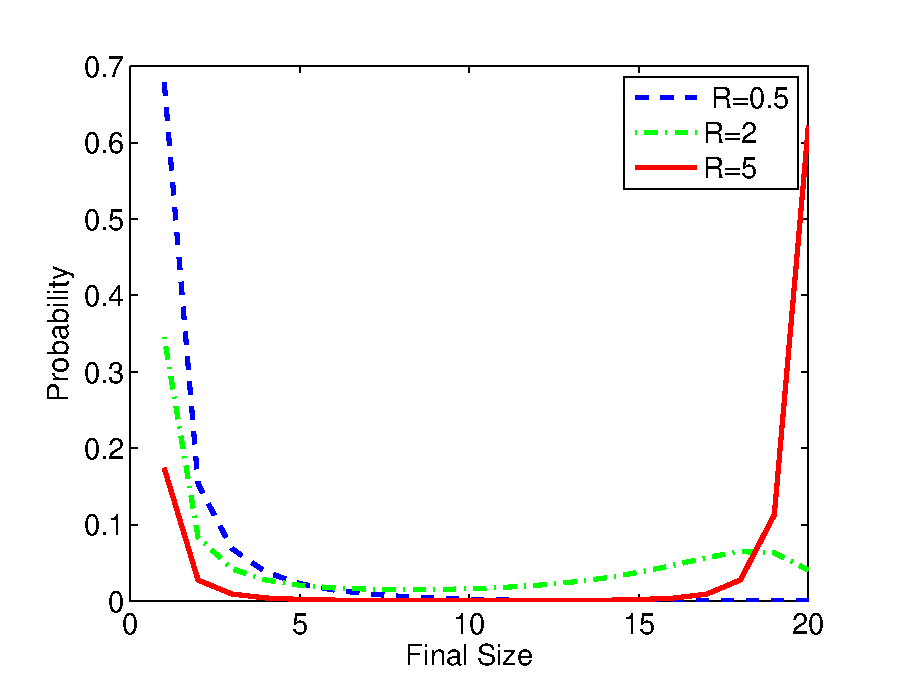
\includegraphics[height=3in,width=3.5in]{DistFinalSize_N20.eps}
}
\subfloat[$N = 100$]{\label{fig:DistributionFinalSize2}
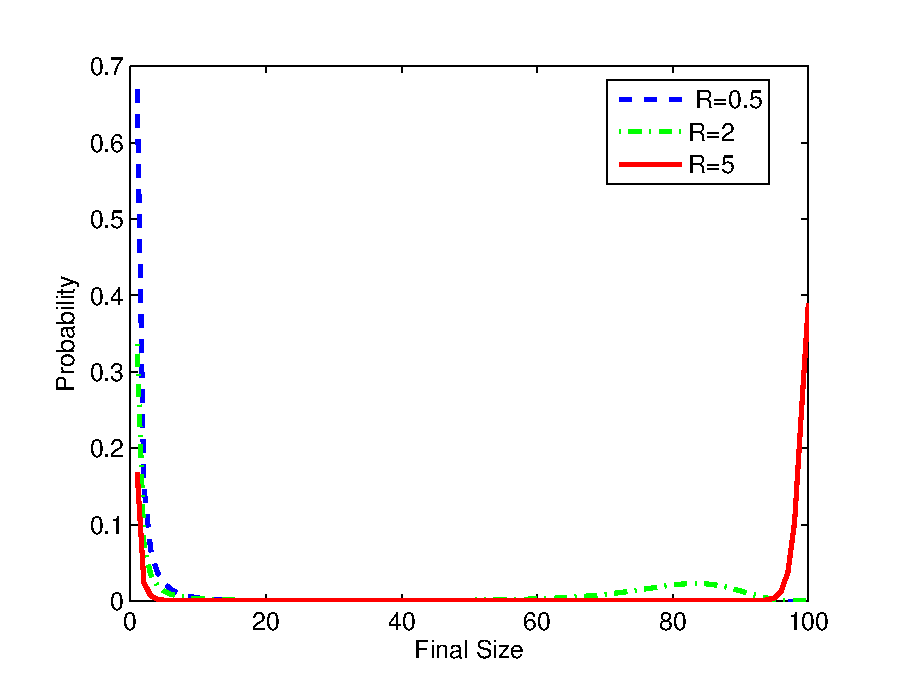
\includegraphics[height=3in,width=3.5in,angle=0]{DistFinalSize_N100.eps}
}
\caption{Probability distribution for final size of stochastic SIR epidemic model when $I(0)=1, S(0)=N-1, \gamma = 1, \beta = 0.5,2,5$}
\label{fig:DistributionFinalSizes}
\end{center}
\end{figure}
%
%
%%%%%%%%%%%%%%%%%%%%			example: final size of distribution		%%%%%%%%%%%%%%%
%
%
\subsection{Example}
To compare with the deterministic case, we tabulate the final size of the stochastic SIR epidemic using the same values for $\gamma$, $S(0)$, $I(0)$. These values should be compared to table~\ref{Table_DetFinalSize} to see that there is disagreement between the two methods. This is due to the fact that in the stochastic case, there is a positive probability that no epidemic will occur and for the deterministic model a disease-free equilibrium is always achieved.
\begin{table}[ht]
	\begin{tabular}{|c||ccc|}
		\hline
	 	   &           &    N       &			\\ \cline{2-4}
	$\beta$ &  $20$ & $100$  	& $1000$   		\\
	\hline
	0.5 & 1.75	& 1.92 	& 1.99   		\\
	1   & 3.36 	& 6.12 	& 13.49  		\\
	2   & 8.19 	& 38.81 	& 215.51 		\\
	5   & 15.63 	& 80.46 	& 211.84  		\\
	10  & 18 	& 90.10 	& 156.92  		\\
	\hline
	\end{tabular}
	\caption{Stochastic SIR: Final Size of Epidemic}
	\label{Table_StochFinalSize}
\end{table}
%
%
%%%%%%%%%%%%%%%%%%%%			STOCHASTIC SIR: EXPECTED DURATION OF AN SIR EPIDEMIC		%%%%%%%%%%%%%%%
%
%
\subsection{Expected Duration of an SIR Epidemic}
We can calculate an expected duration for the stochastic SIR epidemic. We let $\tau _{(s,i)} $ be the expected duration of the SIR epidemic given $ s $ susceptibles and $ i $ infectives. It is clear that $\tau  _{(s,i)} = 0  $ since an epidemic cannot occur, much less endure, if there are no infectives in the population at time zero. It will be stated here without proof that $\tau _{(s,i)}$ satisfies:

\begin{equation*}
\tau _{(s,i)}  = \eta _{si} + p_s \tau _{(s,i-1)} + (1-p_s) \tau _{(s-1,i+1)}
\end{equation*}

The term $\eta _{si}$ is the mean inter-event time given that the state of the process is $(s,i)$, with $s=0,1,2,...,N$ and $i=1,2,...N-s$. It is defined as $\eta _{si} = 1/ \left [ \gamma i + (\beta /N) si    \right ]   $. Substituting for $\eta _{si}$ and rearranging terms gives:
\begin{equation}
\left [ \gamma i + ( \beta / N) s i \right ] \left [ p_s \tau _{(s,i-1)} - \tau _{(s,i)} + (1-p_s) \tau _{(s-1,i+1)} \right ]  = -1
\end{equation}

This system of equation is linear, taking the form $D \tau = \text{\bf d} $, where D is an $\frac{(N+1)(N+2)}{2} \times \frac{(N+1)(N+2)}{2}$   invertible matrix. The expected duration, $\tau$, is then determined by $\tau = D^{-1} \text{\bf d}$.

For a stochastic SIR process with $N=100$, $\beta = 2$, and $\gamma = 1$ estimated distributions for the duration are displayed in Figure~\ref{fig:DistributionDurations} for the initial conditions $I(0)=1$ and $I(0)=5$. We see that for the case $I(0)=1$ the distribution is skewed to the left; that is, the epidemic is not likely to last very long, which is what one would suppose for a disease carried by only a single person. For the case $I(0)=5$, there are more infectives who can transmit the disease to others, and so the epidemic can reasonably be expected to endure longer. This is illustrated in figure~\ref{fig:DistributionDuration2}.

\begin{figure}[ht]
\begin{center}
\subfloat[$I(0) = 1$ and $S(0)=99$]{\label{fig:DistributionDuration1}
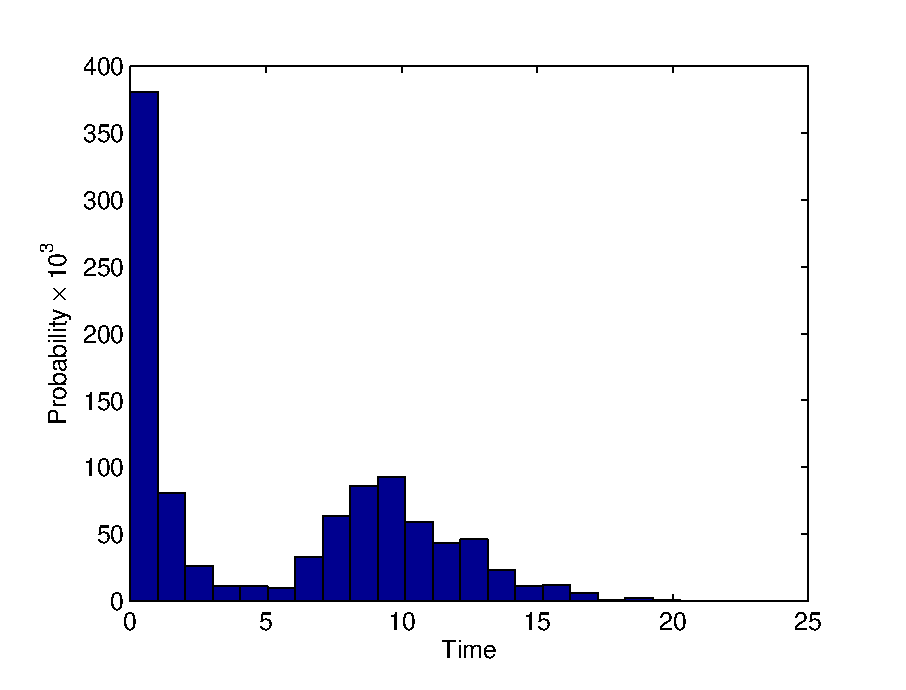
\includegraphics[height=3in,width=3.5in]{DurationDistribution_1Infectives.eps}
}
\subfloat[$I(0) = 5$ and $S(0)=95$]{\label{fig:DistributionDuration2}
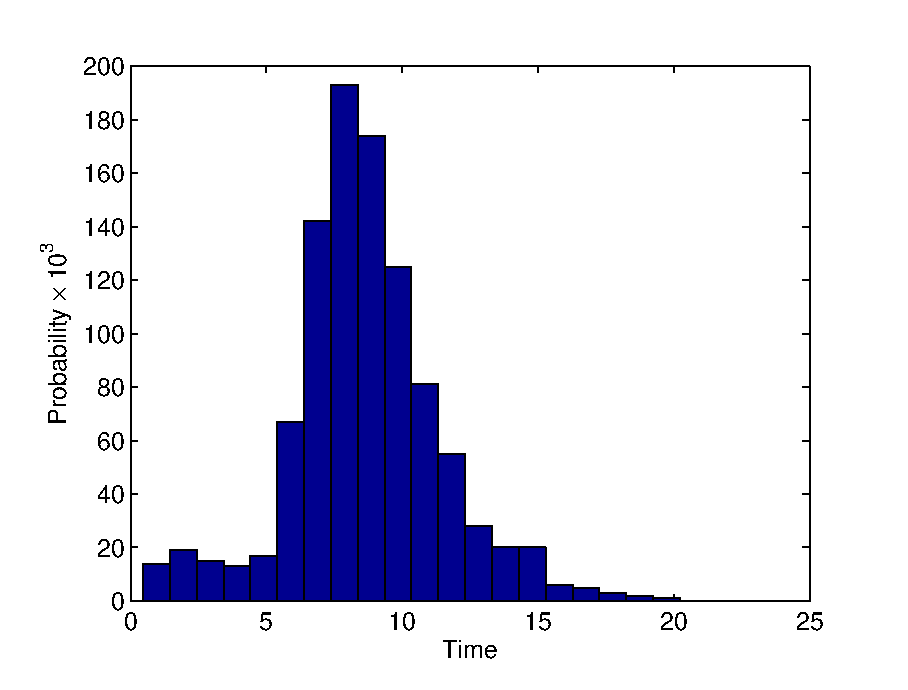
\includegraphics[height=3in,width=3.5in,angle=0]{DurationDistribution_5Infectives.eps}
}
\caption{Probability Distribution for duration of stochastic SIR epidemic (1,000 realizations)}
\label{fig:DistributionDurations}
\end{center}
\end{figure}
%
%
%%%%%%%%%%%%%%%%%%%%						SUMMARY						%%%%%%%%%%%%%%%%%%%
%
%
\section{Summary}
The deterministic and stochastic SIR model without vital dynamics was reviewed. In the deterministic case, it was found that the value of the effective reproduction number $\mathcal R$ determines the occurrence of an epidemic, with $\mathcal R > 1$ leading to an epidemic and $\mathcal R \le 1$ assuring that an epidemic will be avoided. The model relies on assumptions that are not necessarily realistic, such as a uniformly mixing population, but it does provide useful insight into the general nature of epidemics for large populations. The stochastic SIR model addresses some of the issues with the deterministic formulation. Since it considers the state variables as discrete, it is able to describe epidemics in small populations. Additionally, the stochastic model provides a probability that an epidemic occurs, given initial conditions, so that even when an epidemic is guaranteed under the deterministic model, one may not necessarily transpire in the stochastic framework. This is more realistic. In the deterministic setting, one may predict the exact total number of infections during an epidemic; realistically there should be a distribution associated with this final size. It was seen that the stochastic model provides a probability distribution for the final size of the epidemic. The stochastic formulation of the SIR epidemic model, which allows for uncertainty in the spread of disease, is the better, more realistic model.

\newpage
%
%
%%%%%%%%%%%%%%%%%%%%						REFERENCES					%%%%%%%%%%%%%%%%%%%
%
%
\section{References}

Allen, L.J.S. ``An Introduction to Stochastic Epidemic Models" in Mathematical Epidemiology, ed. Brauer F. et al. Springer, 2008. 81-130.

Allen, L.J.S. An Introduction to Stochastic Processes with Applications to Biology. Pearson Education Inc./Prentice Hall, New Jersey (2003)

Allen, L.J.S. Comparison of deterministic and stochastic SIS and SIR models in discrete time. Math Biosci., {\bf 163}, 1-33. (2000)

Daly, D.J., Gani J.: Epidemic Modeling: An Introduction. Cambridge Studies in Mathematical Biology, Vol 15. Cambridge University Press, Cambridge (1999)

Earn, D.J.D. ``A Light Introduction to Modelling Recurrent Epidemics" in Mathematical Epidemiology, ed Brauer F. et al. Springer, 2008. 81-130.

Hethcote, H.W. Qualitative Analyses of Communicable Disease Models, Math. Biosci. {\bf 28}, 335-356 (1976)

Murray, J.D. Mathematical Biology I: An Introduction. New York, Springer-Verlag, 2001.
%
%
%%%%%%%%%%%%%%%%%%%%						APPENDIX					%%%%%%%%%%%%%%%%%%%
%
%

\end{document}